\documentclass[10pt,a4paper]{article}

\usepackage[T1]{fontenc}
\usepackage[utf8]{inputenc}
\usepackage[french,english]{babel}
\usepackage[osf]{newtxtext}

\usepackage[hyphens]{url}
\usepackage{hyperref}
\DeclareUrlCommand\email{\urlstyle{rm}}

\usepackage[margin=2in]{geometry} % showframe
\usepackage{multicol}

\usepackage{graphicx}
\usepackage{xcolor}
\usepackage{amsmath}
\usepackage{amsthm}
\usepackage{amsfonts}
\usepackage{amssymb}
\usepackage{siunitx}
\usepackage{pdflscape}
\usepackage{listings}
\usepackage{float}
\usepackage{pmboxdraw}
\usepackage{float}

\usepackage{todonotes}
\usepackage{marginnote}
\let\marginpar\marginnote

% hyperref setup
\definecolor{darkgreen}{RGB}{0,180,0}
\hypersetup{
    colorlinks = true,
    linkbordercolor = {white},
    linkcolor = red,
    anchorcolor = black,
    citecolor = darkgreen,
    filecolor = cyan,
    menucolor = black,
    runcolor = cyan,
    urlcolor = magenta
}

% Bib setup
\usepackage{csquotes} % Recommended by biblatex
\usepackage[style=numeric,sorting=none,backend=biber]{biblatex}
\DeclareBibliographyAlias{software}{online}
\addbibresource{references.bib} % The file containing our references, in BibTeX format


\newcommand{\htriple}[3]{\ensuremath{\{#1\}~#2~\{#3\}}}
\newcommand{\WP}{\ensuremath{\mathit{WP}}}
\newcommand{\notimplies}{%
  \mathrel{{\ooalign{\hidewidth$\not\phantom{=}$\hidewidth\cr$\implies$}}}}
\newcommand{\eqdef}{\stackrel{def}{=}}

% \renewcommand{\implies}{\ensuremath{\Rightarrow}}

\newtheorem{theorem}{Theorem}[section]
\newtheorem{corollary}{Corollary}[theorem]
\newtheorem{lemma}[theorem]{Lemma}
\newtheorem{remark}{Remark}
\newtheorem*{remark*}{Remark}

%% Listing settings
\definecolor{codegreen}{rgb}{0,0.6,0}
\definecolor{codegray}{rgb}{0.5,0.5,0.5}
\definecolor{codepurple}{rgb}{0.58,0,0.82}
\definecolor{codeblue}{rgb}{0.10,0,0.82}
\definecolor{codebackcolour}{rgb}{0.95,0.95,0.92}


\title{Experiments on automation of formal verification of devices at the binary level}
\author{Thomas Lacroix --- \email{thomas.lacroix@insa-lyon.fr}\medskip\\
Département Informatique\\
INSA de Lyon}
\date{2018/2019}

\begin{document}

\newgeometry{margin=2cm}

\maketitle
\thispagestyle{empty}

{
\noindent Sous la responsabilité de :\\
Mads Dam : Division of Theoretical Computer Science -- KTH\\
Pierre-\'Edouard Portier : Département Informatique -- INSA Lyon
}

\vspace{\baselineskip}\vspace{\baselineskip}

{ % Block used for font size in abstracts
\fontsize{9}{10.8}

\begin{abstract}
  \rightmargin=1cm \leftmargin=1cm
  With the advent of virtualization, more and more work is being dedicated to the verification of hypervisors at the binary level. Platforms are being developed to assist in this verification, but much of the work remains manual.

  In this thesis, we use the HolBA platform and its intermediate representation language BIR for the formal verification of a Network Interface Controller (NIC). The objective is to automate and reduce the repetitive work of an existing proof.

  First, we replaced the formal NIC model with an equivalent one written in BIR. Then, we used Hoare Triples in conjunction with an SMT solver to perform contract-based verification. Finally, we proved formally a simple contract on a BIR implementation, paving the way for more complex proofs with the HolBA platform. Visualization tools have also been implemented when required.
\end{abstract}

\leftmargin=1cm
{\small\textbf{\textit{Keywords---}} binary analysis, formal verification, proof-producing analysis}

\vspace{\baselineskip}\vspace{\baselineskip}

\begin{otherlanguage}{french}
  \begin{abstract}
    \rightmargin=1cm \leftmargin=1cm
    Avec la démocratisation de la virtualisation, de plus en plus d'efforts sont consacrés à la vérification au niveau binaire des hyperviseurs. Des plates-formes sont en cours de développement pour aider cette vérification, mais une grande partie du travail est encore manuelle.

    Nous utilisons ici la plate-forme HolBA et son langage de représentation intermédiaire BIR pour la vérification formelle d'un Contrôleur d'Interface Réseau (NIC). L'objectif est d'automatiser et de réduire le travail répétitif d'une preuve existante.

    Nous avons d'abord remplacé le modèle formel du NIC par un modèle équivalent écrit en BIR. Ensuite, nous avons utilisé des triplets de Hoare en conjonction avec un solveur SMT pour effectuer des vérifications par contrat. Enfin, nous avons prouvé formellement un contrat simple sur une implémentation en BIR, ouvrant la voie à la réalisation de preuves plus complexes avec la plate-forme HolBA. Des outils de visualisation ont également été implémentés selon les besoins rencontrés.
  \end{abstract}
\end{otherlanguage}

\leftmargin=1cm
{\small\textbf{\textit{Mot-clés---}} analyse binaire, vérification formelle, génération de preuves}
}

\vspace{\baselineskip}\vspace{\baselineskip}

\restoregeometry
\newgeometry{margin=3cm}
\fontsize{10}{12}\selectfont
%--------------------------

\begin{multicols}{2}

%%%%%%%%%%%%%%%%%%%%%%%%%%%%%%%%%%%%%%%%%%%%%%%%%%%%%%%%%%%%%%%%%%%%%%%%%%%%%%%%
%%%%%%%%%%%%%%%%%%%%%%%%%%%%%%%%%%%%%%%%%%%%%%%%%%%%%%%%%%%%%%%%%%%%%%%%%%%%%%%%
%%%%%%%%%%%%%%%%%%%%%%%%%%%%%%%%%%%%%%%%%%%%%%%%%%%%%%%%%%%%%%%%%%%%%%%%%%%%%%%%
%%%%%%%%%%%%%%%%%%%%%%%%%%%%%%%%%%%%%%%%%%%%%%%%%%%%%%%%%%%%%%%%%%%%%%%%%%%%%%%%

\section{Introduction}

\subsection{Background}

Embedded systems are becoming more and more common with the current advent of {IoT} and mobile computing platforms, such as smartphones. Those systems are fully-fledged computers with powerful hardware, complete operating systems, and access to the Internet. Such systems can run security-critical services, such as a building security system or automatic toll gates, or carry valuable information as it is the case for personal smartphones. Therefore, these two characteristics make them targets of choice for attackers.

The {PROSPER} project \cite{noauthor_prosper:_nodate-1} aims to develop a secure and formally verified hypervisor for embedded systems. Hypervisors are thin layers running directly on top of hardware providing the ability to run virtualized applications, such as operating systems or real-time control systems. Those virtualized applications then don't have privileged access to the hardware and have to go through the hypervisor. This allows different applications to share the same hardware while providing strong isolation between them, thus ensuring confidentiality and security. Moreover, security not only means protection from external attacks but also resilience to bugs. If multiple critical systems are running on the same hardware, bugs or crashes in some systems shouldn't affect others from behaving correctly.

Previous work in the {PROSPER} project achieved to formally verify a simple separation kernel \cite{dam_formal_2013}, which later resulted into an implementation of a working hypervisor. Then, they formally verified memory isolation for virtualized applications \cite{nemati_trustworthy_2015}. However, hardware devices were not included in the verification, so devices, like Network Interface Controller ({NIC}), cannot be used by virtualized applications. Thid reduces the value of the hypervisor. In order to solve this issue, verification of hardware devices is being carried out.

A formal model of a {NIC} device has been produced, on which some security theorems have been proved \cite{haglund_formal_2016,haglund_trustworthy_nodate}. These theorems can be seen as high-level proofs relying on multiple layers of lower-level lemmas. This is illustrated in the left-hand side of Figure \ref{hol-v-bir-nic-model-simple}. However, there exist more devices that are of interest to verify, so it is very desirable to automate formal verification of devices and use a standard model for reasoning about them.
%
\begin{figure}[H]
  \centering
	\includegraphics[height=6cm]{figures/hol-v-bir-nic-model-simple.png}
	\caption{Formal vs. BIR NIC models. The left hand side already exists. The dashed elements represent the work done during this project.}
	\label{hol-v-bir-nic-model-simple}
\end{figure}

The team is now developing a new platform named {HolBA} for performing binary analysis in HOL4, an interactive theorem prover. This platform features a machine-independent Binary Intermediate Representation (BIR), a proof-producing transpiler from ARMv8 and Cortex-M$0$ assembly code to BIR, called the ``lifter'', a proof-producing weakest precondition generator for loop-free programs, and some supporting tools \cite{metere_sound_2017,lindner_trabin:_2019}.

The idea of this work is to translate the formal {NIC} model of \cite{haglund_formal_2016} using {BIR}, then use HolBA's proof-producing weakest precondition tool to prove the same lower-level lemmas as the formal model. With all the lemmas proved, the security properties are implied. Figure \ref{hol-v-bir-nic-model-simple} gives an overview of this idea.

\subsection{Thesis objective}

The goal of this thesis project is to explore verification techniques in order to automate parts, if not all, of the verification process of hardware devices using the HolBA platform. The formal {NIC} model of \cite{haglund_formal_2016} is used as working example.

\subsection{Delimitations}

This work being about exploration of techniques towards automation of verification techniques, instead of being about producing an actual complete proof of a hardware device, some implementations have not been completed in order to save time to explore in more areas. Additionally, this work concerned mainly the HolBA platform that is developed in the team where this thesis took place.

\subsection{Choice of methodology}

This work has been carried out step-by-step towards an ideal goal, i.e. re-establishing all the security properties. On the road, needs have been identified and tools have been implemented in order to tackle them. This approach made sense in this particular work because the needs were not known in advance, and therefore needed to be identified. This document presents the steps taken during this work, the motivations of each tool that have been implemented, and discusses their limitations and future work in the conclusion.

\subsection{Related work}

\subsubsection{Secure execution platforms}

The {PROSPER} project isn't the only project focused on high-security execution platforms. Platforms such as seL4, Microsoft Hyper-V, INTEGRITY Multivisor or even MINIX 3 are examples of platforms used in production that are providing strong security properties.

Each of these projects intends to provide a secure hypervisor or operating system, but they all provide different levels of guarantee. seL4 is an open-source microkernel that has been formally verified down to binary code. Microsoft's hypervisor, Hyper-V, has also been verified down to its machine code, but with less trustworthy tools than seL4 because of its huge codebase. MINIX 3 rather intends to give security properties by design by giving the least responsibilities to the microkernel. INTEGRITY Multivisor doesn't provide much public information, but has had considerable formal verification and has got several industry and military certifications. However, to the best of our knowledge, none of these platforms include hardware devices in their formal verification process other than by their design.

\subsubsection{Binary analysis platforms}

For this project, we used the {HolBA} platform. However, several other binary analysis platforms have already been created for various purposes, such as formal verification or static analysis. A common characteristic of these platforms is their use of an Intermediate Representation ({IR}). IRs are designed to be simpler to use for each platforms' end purpose. HolBA has BIR as its intermediate representation.

Microsoft has Boogie as both a tool and IR, which has been used for verification of {Hyper\nobreakdash-\hspace{0pt}V}. Valgrind is a popular framework for building program supervision tools, and uses a JIT x86-to-x86 compiler in order to transpile program to its IR. LLVM is a compiler infrastructure built around LLVM Virtual Instruction Set, its {IR}, that links together an ecosystem of tools at multiple stages of the compilation process, including verification and analysis. Mayhem is a system for automatically finding exploitable bugs in binary programs, and leverages Carnegie Mellon University Binary Analysis Platform (CMU BAP). An interesting note though is that BIR's design is based upon CMU BAP's IR.

The novelty introduced in HolBA, however, is that proofs are performed, directly on the generated assembly code, not at the source code level. Therefore, programs can be analyzed without their source code, and regardless on the programming language used as long as it can be compiled in assembly code in an Instruction Set Architecture ({ISA}) supported by the platform.

% Note: Mayhem does work at binary level, but it doesn't produce proofs. It finds exploits but doesn't garantee their absence.

%%%%%%%%%%%%%%%%%%%%%%%%%%%%%%%%%%%%%%%%%%%%%%%%%%%%%%%%%%%%%%%%%%%%%%%%%%%%%%%%
%%%%%%%%%%%%%%%%%%%%%%%%%%%%%%%%%%%%%%%%%%%%%%%%%%%%%%%%%%%%%%%%%%%%%%%%%%%%%%%%
%%%%%%%%%%%%%%%%%%%%%%%%%%%%%%%%%%%%%%%%%%%%%%%%%%%%%%%%%%%%%%%%%%%%%%%%%%%%%%%%
%%%%%%%%%%%%%%%%%%%%%%%%%%%%%%%%%%%%%%%%%%%%%%%%%%%%%%%%%%%%%%%%%%%%%%%%%%%%%%%%

\subsection{Definitions and relevant theories}

\subsubsection{Interactive Theorem Proving and HOL4} \label{hol4-presentation}

Interactive theorem provers are software producing formal proofs, in an
interactive fashion, i.e. a human can step through the proof interactively while the proof assistant provides some automation (like rewriting of terms, arithmetic evaluation, or integration with external tools like SMT solvers). Coq, HOL4 or Isabelle are such tools.

HOL4 stands for Higher-Order Logic. It is a programming environment deeply embedded into the {SML} programming language enabling to prove theorems and write {proof-producing} programs. HOL4 uses a very small kernel in order to provide very high guarantees of correctness.

\subsubsection{HolBA's BIR} \label{bir-presentation}

BIR is a machine independent binary representation. It aims to be simple while still being able to represent all possible binary programs except self-modifying programs. It does so by having a limited syntax and by forbidding implicit side-effects. A statement can only have explicit state changes and can only affect one variable.

This representation makes producing proofs easier than with classical binary representations, whose design are focused on execution speed rather than offline analysis.

BIR is implemented as a set of HOL4 data types, and possesses a completely defined semantics.

% Among its supporting tools, HolBA features a tool to visualize the Control Flow Graph ({CFG}) of BIR programs.

\subsubsection{Hoare Triples} \label{hoare-triples}

For a given program $prog$ consisting of a list of instructions, and two predicates $P$ and $Q$ called respectively pre- and postcondition, a Hoare Triple \htriple{P}{prog}{Q} states that when executing the program $prog$ from a state $S$ terminates in a state $S'$, if $P$ holds in $S$ then $Q$ will hold in $S'$ (Equation \ref{ht_def}). A Hoare Triple is also called \textit{a contract}.
%
\begin{multline}
  \htriple{P}{prog}{Q} \eqdef\\
  S' = exec(S, prog) \land P(S) \implies Q(S')
  \label{ht_def}
\end{multline}

For example, \htriple{P}{\varnothing}{P} holds because an empty program doesn't change the state of the execution. \htriple{n=1}{n:=n+1}{even(n)} with $n \in \mathbb{N}$ holds because $1+1=2$, which is even.

\subsubsection{Weakest preconditions}

While Hoare Triples introduce sufficient preconditions, Dijkstra introduced the concept of necessary and sufficient preconditions, called ``weakest'' preconditions (WP) \cite{dijkstra_guarded_1975}. WP can be automatically derived from a program $prog$ and a postcondition $Q$. Let's call $\WP(prog, Q)$ such a WP. Then, from Equation \ref{ht_def} follows:
%
\begin{equation}
  \forall (prog, Q),
  \htriple{\WP(prog,Q)}{prog}{Q}
  \label{ht_wp_eq}
\end{equation}

For the program $n:=n+1$ mentioned in the previous section, the WP for the postcondition $even(n)$ is $odd(n)$, i.e. incrementing the value of an odd integer variable by one makes it even.

For a triple \htriple{P}{prog}{Q} to hold, $P$ must be stronger than the WP, i.e. we need to prove that $P \implies \WP(prog, Q)$. While multiple methods exist to perform such proofs, Satisfiability Modulo Theory ({SMT}) solvers offer a convenient and automatic solution. With an SMT solver, proving $R$ consist in checking that $\neg R$, its negation, is \textit{unsatisfiable}. SMT solvers can also give counter-example if $R$ is false.

{HolBA} provides a {proof-producing} tool for automatically deriving WP on loop-free {BIR} programs whose control-flow can be statically identified \cite{lindner_trabin:_2019}. However, SMT solvers had never been used with HolBA before this work.

%%%%%%%%%%%%%%%%%%%%%%%%%%%%%%%%%%%%%%%%%%%%%%%%%%%%%%%%%%%%%%%%%%%%%%%%%%%%%%%%
%%%%%%%%%%%%%%%%%%%%%%%%%%%%%%%%%%%%%%%%%%%%%%%%%%%%%%%%%%%%%%%%%%%%%%%%%%%%%%%%
%%%%%%%%%%%%%%%%%%%%%%%%%%%%%%%%%%%%%%%%%%%%%%%%%%%%%%%%%%%%%%%%%%%%%%%%%%%%%%%%
%%%%%%%%%%%%%%%%%%%%%%%%%%%%%%%%%%%%%%%%%%%%%%%%%%%%%%%%%%%%%%%%%%%%%%%%%%%%%%%%

\section{Overview of the formal proof of the NIC model} \label{overview-nic-proof}

The formal verification of \cite{haglund_formal_2016} represents the NIC as a transition system. It is composed of five finite state automata, each responsible for a different task: initialization, transmission, transmission teardown, reception and reception teardown. These automata have autonomous transitions that represent the standalone operation of the device. Communication with the CPU is represented with non-autonomous transitions. The model also contains a scheduler. Since this model has been realized using the public specification of the device, which is underspecified, the simulated state of the device is marked \textit{dead} if the model is asked to describe any transition or operation that is not described by the specification.
Being designed as a transition system, the whole model is loop-free. This is convenient for contract-based verification because composition theorems would otherwise be needed.

The state of the NIC is defined as a nested data type containing registers and a memory called \textit{CPPI\_RAM}.

The low-level lemmas of the verification (cf. Figure \ref{hol-v-bir-nic-model-simple}) are stated as Hoare Triples using invariants that must hold for every possible transition:
%
\begin{small}
  \begin{equation}
    \label{nic-proof-invariant-shape}
    I_{NIC} \eqdef \neg NIC.dead~\land~I_{init}~\land~I_{tx}~\land~I_{td}~\land~I_{rx}~\land~I_{rd}
  \end{equation}
\end{small}

\subsection{Visualizing proof dependencies}

The model of the NIC consists of \num{1500} lines of HOL4 code and required around three man-months of work. The NIC invariant consists of \num{650} lines of HOL4 code and the proof consists of approximately \num{55000} lines of HOL4 code including comments. Identifying the invariant and implementing the proof in HOL4 required around one man-year of work \cite{haglund_trustworthy_nodate}.

The proof being large and divided into several script files, it is difficult to identify what are the low-level lemmas to be reproved in this work. Therefore, a tool, called DepGraph, has been implemented in order to extract the dependency structure from proof files in the form of a graph. Then, the fringe of the graph represents the smallest set of lemmas that is enough to prove in order to imply the security properties by using the rest of the proofs unchanged.

DepGraph features two frontends that can extract dependencies between HOL4 theories (i.e. compiled {SML} files containing proofs of lemmas and theorems), and between definitions, theorems, and lemmas. However, this tool presents some critical shortcomings:

\paragraph{The theory dependencies frontend} uses files generated by Holmake, the HOL4 compile system, in order to get the dependencies between theories. However, those files don't really represent dependencies but the files to be loaded before this script can be loaded, in a recursive fashion. Therefore, they represent the transitive reduction of the dependency graph. Because of this, precious knowledge is lost and cannot be recovered by using this method: edges representing direct dependencies are removed if the remaining edges still account for this dependency. Therefore, we are still able to tell which nodes depend on some node $n$, but we cannot identify the aforementioned fringe. In order to solve this problem, different approaches exist, such as implementing a simplified SML parser that looks only at dependencies, or injecting code inside the dependency resolution of an existing SML compiler. However, this would involve too much work that isn't the direct focus of this thesis.

\paragraph{The definition, theorem and lemma dependencies frontend} uses word-based heuristics in order to extract dependencies, and is as such not quite reliable and cannot give any guarantee. As above, there exist similar solutions in order to get multiple levels of guarantees, such as implementing a SML parser or injecting code inside HOL4 theory and definitions handling, but this would also require too much work. Destructuring theories does not work because of how HOL4 has been designed. Moreover, such dependency graphs become quickly big, making them unusable in practice. Therefore, no further work has been put into this frontend.

\medskip
DepGraph's frontend for theory dependencies is still useful for documentation purpose, and has been used to visualize HolBA's architecture.

%%%%%%%%%%%%%%%%%%%%%%%%%%%%%%%%%%%%%%%%%%%%%%%%%%%%%%%%%%%%%%%%%%%%%%%%%%%%%%%%
%%%%%%%%%%%%%%%%%%%%%%%%%%%%%%%%%%%%%%%%%%%%%%%%%%%%%%%%%%%%%%%%%%%%%%%%%%%%%%%%
%%%%%%%%%%%%%%%%%%%%%%%%%%%%%%%%%%%%%%%%%%%%%%%%%%%%%%%%%%%%%%%%%%%%%%%%%%%%%%%%
%%%%%%%%%%%%%%%%%%%%%%%%%%%%%%%%%%%%%%%%%%%%%%%%%%%%%%%%%%%%%%%%%%%%%%%%%%%%%%%%

\section{The BIR NIC model} \label{nic-model}

Three approaches to the translation of the formal NIC model to an equivalent BIR program have been considered, from handwritting a BIR program (Sections \ref{alice-bob-toy} to \ref{impl-real-model}), lifting a C program (Section \ref{c-model}), to developing a new device-model-specific IR (Section \ref{flowchart-attempt}).

\subsection{Using flowcharts as IR} \label{flowchart-attempt}

The Control Flow Graph ({CFG}) of the transition system of the formal model looks like a tree. Therefore, using flowcharts could be a convenient way to represent such structures. An attempt has been made to design a flowchart representation.

While this visual representation is useful in order to get to know the formal NIC model, we encountered several shortcomings:

\paragraph{Flowcharts of each transition rapidly grow in size} with the complexity of its formal counterpart. Possible workarounds include the use of nested diagrams or usage of shorter ways of representing common patterns.

\paragraph{Coherent visual language are hard to design} to represent the full set of features needed in order to realize device models. Additionally, this language must be compatible or easily translatable to BIR.

\paragraph{It is hard to design a textual representation} of this visual language other than conventional programming languages, so using such representation would require a substantial implementation effort in order to implement all the tools needed to use it. Developing visualization tools for a conventional language appears to be a more reasonable approach than developing a visual language.

\medskip
For those reasons, we decided to not go further with this visual representation, and to focus instead on existing tools of the HolBA platform.

\subsection{Writing the model in C} \label{c-model}

One-to-one translation of the definitions related to the transmission automaton, scheduler, state, and \textit{CPPI\_RAM} of the formal model have been realized in C. However, when studying the compiled assembly code and lifted BIR program, we noticed that all the convenient naming that we can use in the formal or the C model is lost and replaced with abundant usage of the stack. While this is completely normal behaviour for a C compiler, this is not convenient when performing later proofs on the model. Reasoning about the stack would require more code than a complete rewrite of the model in BIR. This experiment made us realize that writing the model is a rapid operation and that we should rather focus on making the verification step as smooth as possible.

\subsection{A toy BIR model} \label{alice-bob-toy}

Before writing the whole NIC model by hand, we shall identify the structure of the model and develop tools that facilitate its implementation. Well-designed tools can reduce the boilerplate work of the implementation, help focus only on the meaningful content, and reduce the chance of introducing bugs as the code is factored and mechanically shorter.

A transition system similar to the one of the NIC model has been implemented, containing one scheduler and two automata. The two automata feature a simple linear transition system. Each of them has one non-autonomous transition that represent memory accesses from the CPU.

This toy model has first been designed using the flowchart representation. Then, writing the BIR program has been a repetitive but straightforward step. The resulting BIR program is \num{450} lines of code long. Two issues have been identified:

\begin{itemize}
    \item BIR, as a HOL4 embedded language, is very verbose. Simple operations like additions or assignments require long constructions. Section \ref{bsl} presents BSL, a less verbose way of writing BIR programs.
    \item BIR features only one conditional statement controlling the control flow of a program: conditional jumps. Hence, BIR is not convenient for representing \textbf{if-then-else} statements with more than two branches.
\end{itemize}

\subsection{BSL: BIR Simple Language} \label{bsl}

A library, named BSL, offering the same expressiveness as BIR but with shorter constructs, has been implemented. This library has been kept simple and will serve as the base layer of possible later abstractions. As such, it has been decided that no feature other than pure syntactic construct, such as type inference, would be included.

BSL is composed of a set of functions with short names (prefixed with the letter \textit{b} in order to not clash with names in the global namespace), a coherent interface offering interoperability with HOL4 quotation system, and smart use of partial function application (e.g. for BIR types).

\subsection{Implementing the real model} \label{impl-real-model}

From the knowledge gained in \ref{alice-bob-toy}, a set of helper functions has been implemented, mainly in order to facilitate reasoning about the state machine.

Because of time constraints, not every transition of the formal NIC model have been implemented. Instead, we decided to focus on only some transitions in two automata: initialization and transmission. This focus is pragmatic for two reasons: (a) we decided to only write the transitions needed for the current proof, in order to grow the model at a reasonable pace; (b) as the verification was performed at the same time, we decided to start with easier, but not obvious, transitions, hence the choice to postpone verification of the more complex reception automaton to later in the work.

%%%%%%%%%%%%%%%%%%%%%%%%%%%%%%%%%%%%%%%%%%%%%%%%%%%%%%%%%%%%%%%%%%%%%%%%%%%%%%%%
%%%%%%%%%%%%%%%%%%%%%%%%%%%%%%%%%%%%%%%%%%%%%%%%%%%%%%%%%%%%%%%%%%%%%%%%%%%%%%%%
%%%%%%%%%%%%%%%%%%%%%%%%%%%%%%%%%%%%%%%%%%%%%%%%%%%%%%%%%%%%%%%%%%%%%%%%%%%%%%%%
%%%%%%%%%%%%%%%%%%%%%%%%%%%%%%%%%%%%%%%%%%%%%%%%%%%%%%%%%%%%%%%%%%%%%%%%%%%%%%%%

\section{Non proof-producing automatic contract verification} \label{impl-non-pp-wp-lib}

This section presents the library that has been implemented in this work for automatic contract verification, after discussing about the problems that have been solved in order to build it.

\subsection{Exporting BIR expressions to SMT solvers} \label{exporting-bir-to-smt}

We must be able to export HOL4 goals to external SMT solvers in order to prove the implication needed to prove Hoare Triples. HOL4 features a library for interfacing {SMT} solvers and HOL4, called \textit{HolSmtLib}, using the standard format SMT-LIB 2.0 \cite{barrett_satisfiability_2016}. However, generated WP are BIR expressions and it cannot export them out of the box.

As an intermediate language for formal verification, {BIR} possesses a precise semantics. The semantics of BIR expressions is expressed as a set of definitions describing what are the equivalent operations using HOL4's \textit{wordsTheory} and \textit{combinTheory}.

Because of the complexity of the BIR semantics, we deciced to implement a non proof-producing translation, in order to get more time for other experiments. The obvious downside of such a function is that we now have to trust the translation to be sound because we no longer get any guarantee from the theorem prover, but a proof-producing version can still be implemented later.

\textit{bir\_exp\_to\_words} has been implemented as an exhaustive \texttt{match} statement on the expression type, each type being then translated to the corresponding non-BIR expression. Recursive call is used for nested expressions.

\subsection{BIR memories and SMT} \label{bir-memories-with-smt-solvers}

In order to prove Hoare Triples containing BIR memories, we need to use \textit{combinTheory}. However, it is not supported by \textit{HolSmtLib}. We proceeded in two steps to solve this issue:

\begin{enumerate}
  \item we looked at how to translate BIR memory operations to SMT-LIB 2.0 and found \textit{ArraysEx}. Then, we verified that this translation is sound by checking that \textit{ArraysEx}'s axioms are correct in HOL4.
  \item we extended \textit{HolSmtLib} in order to support this theory, and wrote tests in order to ensure that the implementation is correct, since this library is not proof-producing \footnotemark.
\end{enumerate}

\footnotetext{\textit{HolSmtLib} does have proof-reconstruction capabilities, but they are using an outdated version of Z3, the SMT solver that we used. Furthermore, adding support for \textit{ArraysEx} would require significant work.}

\subsection{Pretty-printing of BIR expressions} \label{pretty-printers}

Generated WP quickly grow in size with the number of statements in a program, linearly or exponentially depending on the type of statements \footnote{Control flow statements produce exponential growth. While clever techniques can be implemented to keep their size reasonable \cite{lindner_trabin:_2019}, we often need to read and analyze them.}. The default printing of BIR terms is very verbose. In order to increase user-friendliness, the readibility of long BIR expressions should be improved. Therefore, we implemented a HOL4 pretty-printer library providing the following features:

\begin{itemize}
    \item Simplification of verbose constructs.
    \item Consistent breaking of long expressions.
    \item Highlighting of types.
    \item Highlighting of labels and variable names.
    \item Gathering of nested binary expressions of the same type at the same level.
    \item Rainbow parenthesis: matching pairs of parenthesis are printed in the same color.
\end{itemize}

\subsection{Implementing a convenient interface} \label{impl_convenient_ht_interface}

In order to perform a high number of proofs on the {NIC} model, we want to hide the implementation details of the contract verification procedure as much as possible. Ideally, we want a function ``\texttt{prove\_contract}'' taking a program fragment, a pre- and a postcondition as parameters, and producing a proof about the Hoare Triple if the contract holds or a comprehensive and useful error message if it doesn't (cf. Section \ref{user-friendliness}).
%
\begin{lstlisting}[
    language=Caml,
    backgroundcolor=\color{codebackcolour},
    keywordstyle=\color{magenta},
    label=interface_prove_contract,caption=Interface of ``\texttt{prove\_contract}'',
    frame=tb,basicstyle=\footnotesize\ttfamily]
fun prove_contract contract_name prog_def
    (precond_lbl, precond_bir_exp)
    (postcond_lbl_list, postcond_bir_exp)
\end{lstlisting}

In order to test this function and check that the interface actually lets us verify different contracts, we verified three different programs:

\begin{enumerate}
  \item we verified \htriple{\top}{prog}{y = 100} on a simple program containing one conditional jump where each target assigns a different value to $y$, but where the condition is always true at runtime.
  \item on a program storing a number $N$ in memory at address $A$, then loading into $x$ from address $B$, we verified \htriple{A=B}{prog}{x=N}. This test allowed us to check if the extension of \textit{HolSmtLib} works.
  \item on a program computing the sum of integers from $0$ to a given $n$ using a for loop, we verified the loop invariant on the body of the loop using Gauss' formula.
\end{enumerate}

For each of those tests, we also experimented with other pre- and postconditions, and checked that invalid contracts cannot be proved.

\subsection{Simple automatized proofs on the NIC model} \label{simple-automated-proofs-on-nic}

The base lemmas of the formal NIC proof are phrased in terms of invariants holding in each transition of the model, representable as Hoare Triples. Hence, they can be proved using the non proof-producing contract verification library, as long as the pre- and postconditions can be represented using BIR.

We used \texttt{prove\_contract} in order to successfully verify two Hoare Triples. They respectively represent that, starting from a non-dead initial NIC state, performing one autonomous transition of the transmission automaton doesn't end in an undefined state (i.e. a dead state) and performing one non-autonomous transition of the initialization automaton does end in an undefined state (Equation \ref{nonpp-goal-2}).
%
\begin{multline}
	\{\neg NIC.dead \land NIC.init.state \in \{it1,it3,it4\}\}\\
	init\_automaton\{NIC.dead\}
    \label{nonpp-goal-2}
\end{multline}

\subsection{Limitations of this approach}

While being convenient and working well for simple contracts, our contract verification library suffers from two limitations:

\paragraph{It isn't {proof-producing}} Using HOL4 requires a significant learning effort, and easier non proof-producing tools exist.

\paragraph{It is limited by the expressiveness of BIR,} since the pre- and postconditions are BIR terms. BIR doesn't have quantifiers, and it is, therefore, impossible to prove contracts containing existential quantifiers. The existing formal proof on the NIC of \cite{haglund_formal_2016} requires existential quantifiers in order to reason about the buffer descriptor queue in the \textit{CPPI\_RAM} memory, so this part of the proof cannot be replaced by using \texttt{prove\_contract}.

\medskip
The following Section \ref{trustful-nic-analysis} explores a new proof-producing approach for performing contract-based verification on the BIR model that gives an answer to these issues.

%%%%%%%%%%%%%%%%%%%%%%%%%%%%%%%%%%%%%%%%%%%%%%%%%%%%%%%%%%%%%%%%%%%%%%%%%%%%%%%%
%%%%%%%%%%%%%%%%%%%%%%%%%%%%%%%%%%%%%%%%%%%%%%%%%%%%%%%%%%%%%%%%%%%%%%%%%%%%%%%%
%%%%%%%%%%%%%%%%%%%%%%%%%%%%%%%%%%%%%%%%%%%%%%%%%%%%%%%%%%%%%%%%%%%%%%%%%%%%%%%%
%%%%%%%%%%%%%%%%%%%%%%%%%%%%%%%%%%%%%%%%%%%%%%%%%%%%%%%%%%%%%%%%%%%%%%%%%%%%%%%%

\section{A new approach for trustful analysis} \label{trustful-nic-analysis}

In order to perform proof-producing analysis on the NIC model, we successfully tried a new approach: we performed a proof on a BIR program and then lifted it to an abstract model. We decided to prove a simple property to show the feasibility of the approach. We used a HOL4 data type composed of two variables, $NIC.dead$ ($bool$) and $NIC.x$ ($word32$), as a formal state on which we want to prove a property. Equations \ref{proof_nic_P_def}, \ref{proof_nic_Q_def} and \ref{proof_goal} present the property that we proved. Listing \ref{proof_prog} contains a pseudocode representation of the BIR program on which we performed the verification. Figure \ref{proof_schema} represents visually the structure of the verification and the steps that we took during the proof.
%
\begin{small}
\begin{align}
  \begin{split}
    \label{proof_nic_P_def}
    \vdash~\forall &nic.~P_{NIC}~nic \eqdef \neg nic.dead \land nic.x = 0w
  \end{split}\\
  %
  \begin{split}
    \label{proof_nic_Q_def}
    \vdash~&\forall nic~nic'.~Q_{NIC}~nic~nic' \eqdef\\
      &~~~~~\neg nic'.dead \land nic'.x = nic.x + 1w
  \end{split}\\
  %
  \begin{split}
    \label{proof_goal}
    \vdash~&\forall nic~nic'.~(exec\_prog~nic~bir\_prog~nic'\\
      &\land~P_{NIC}~nic)~\implies~Q_{NIC}~nic~nic'
  \end{split}
\end{align}
\end{small}
%
\begin{remark} \label{remark_Q_nic_intial_final}
  $Q_{NIC}~nic~nic'$ has been defined on both initial and final states, in order to be able to reason about the initial state in the postcondition. This allowed us to write $nic'.x = nic.x + 1w$ instead of $nic'.x = 1w$.
\end{remark}
%
\begin{lstlisting}[
    language=C,
    backgroundcolor=\color{codebackcolour},
    commentstyle=\color{codegreen},
    keywordstyle=\color{magenta},
    stringstyle=\color{codepurple},
    label=proof_prog,caption=Pseudocode of the program used in this proof,
    frame=tb,basicstyle=\footnotesize\ttfamily]
nic.x := nic.x + 1
if nic.x > 10:
    nic.dead := true
\end{lstlisting}
%
\begin{figure}[H]
	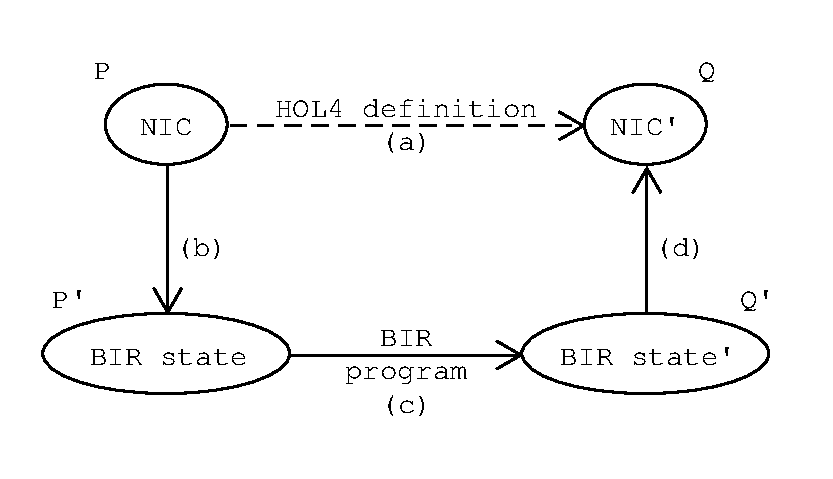
\includegraphics[width=\columnwidth]{figures/proof_schema.pdf}
	\centering
	\caption{Visual structure of the proof. References like (a) to the arrows of this Figure are used to refer to a particular step.}
	\label{proof_schema}
\end{figure}
%
\par We used Definition \ref{proof_eq_thm} in order to establish a relation between the HOL4 definition (a) and the BIR program (c). Another solution would have been to generate a proof-producing lifter from the formal definition (a) to BIR program (c), but has been kept as future work.
%
\begin{small}
  \begin{equation}
  \begin{split}
    \vdash \forall &nic~nic'.~exec\_prog~nic~bir\_prog~nic'~\eqdef ~~ \text{(a)}\\
      &\forall bir\_state~bir\_state'.~(R~nic~bir\_state~\land ~~ \text{(b)}\\
            &~~~~bir\_state' = BIR\_exec~prog~bir\_state) ~~ \text{(c)}\\
            &~\implies R~nic'~bir\_state' ~~~~~~~~~~~~~~~~~~~~~~~~~~~~~~~~~\, \text{(d)}
  \end{split}
  \label{proof_eq_thm}
  \end{equation}
\end{small}
%
\par The relation $R$ is used to express an equivalence between HOL4 states (``$nic$'') and BIR states. It is defined as a mapping of the variables between the BIR state and the formal state.

\begin{proof}

For (b), we proved the injectivity of $R$.

Then, we defined the equivalent pre- and postcondition in BIR, and proved Theorem \ref{proof_b_thm}.
%
\begin{equation} \label{proof_b_thm}
  \begin{split}
  \vdash~\forall bir\_state~(\exists nic.~R~nic~bir\_state~\land\\
  P_{NIC}~nic) \implies P_{BIR}~bir\_state
  \end{split}
\end{equation}

For step (d), we proved Theorem \ref{proof_d_thm}. We introduced $bir\_state$ and $P_{BIR}$ in order to reason about both the initial and final state in the postcondition (cf. Remark \ref{remark_Q_nic_intial_final}).
%
\begin{equation} \label{proof_d_thm}
\begin{split}
\vdash~\forall~&bir\_state'.~Q_{BIR}~bir\_state' \implies\\
	&(\forall nic~nic'~bir\_state.~P_{BIR}~bir\_state\\
	&~\land~R~nic~bir\_state~\land~R~nic'~bir\_state'\\
	&~\implies Q_{NIC}~nic~nic')
\end{split}
\end{equation}
\paragraph{Limitation} \textit{$Q_{BIR}$ is a function of the end state only. Hence, in order to reason about the initial state, we need in general to introduce ghost variables postcondition. In this proof, since the contract that we are proving is simple, using the actual value of $nic.x$ is enough. However, this may pose a problem if we want to generalize the proof.}
\medskip

Finally, we proved that the Hoare Triple holds on the BIR program:
%
\begin{equation} \label{proof_ht_thm}
\vdash~\htriple{P^{exp}_{BIR}}{bir\_prog}{Q^{exp}_{BIR}}
\end{equation}

To that end, we used HolBA's proof-producing WP tool to generate the implication $P \implies WP$ as a BIR expression. Then, to turn the goal into a \textit{wordsTheory} expression, we showed the assumptions needed to use BIR semantics' rewrite theorems about well-typedness and initialization, as well as Lemmas \ref{proof_exists_x_imm} and \ref{proof_exists_x_word} instantiated for all BIR variables. We were then able to rewrite the goal using the full set of BIR semantics theorems and some rewriting rules into a form that \textit{HolSmtLib} can handle.
%
\begin{align}
  \label{proof_exists_x_imm}
  \exists x\_imm.~x\_val = BVal\_Imm~x\_imm\\
  \label{proof_exists_x_word}
  \exists x\_word.~x\_imm = Imm32~x\_word
\end{align}

To complete the proof of Theorem \ref{proof_goal}, we used the deduction rule with the injectivity theorem, Theorem \ref{proof_b_thm}, the definition of $R$, and Theorems \ref{proof_ht_thm}, \ref{proof_eq_thm} and \ref{proof_d_thm}, in that order.
\end{proof}

%%%%%%%%%%%%%%%%%%%%%%%%%%%%%%%%%%%%%%%%%%%%%%%%%%%%%%%%%%%%%%%%%%%%%%%%%%%%%%%%
%%%%%%%%%%%%%%%%%%%%%%%%%%%%%%%%%%%%%%%%%%%%%%%%%%%%%%%%%%%%%%%%%%%%%%%%%%%%%%%%
%%%%%%%%%%%%%%%%%%%%%%%%%%%%%%%%%%%%%%%%%%%%%%%%%%%%%%%%%%%%%%%%%%%%%%%%%%%%%%%%
%%%%%%%%%%%%%%%%%%%%%%%%%%%%%%%%%%%%%%%%%%%%%%%%%%%%%%%%%%%%%%%%%%%%%%%%%%%%%%%%

\section{User experience and good practices} \label{user-friendliness}

\subsection{Towards a better user experience} \label{towards-user-exp}

Throughout our design and implementation process, great care has been taken in order to have a good user experience.

\paragraph{BSL and the pretty-printer} are two successful attempts to simplify HolBA users' manipulation of BIR, respectively writing and reading BIR code. While HOL4 provides powerful quotation and printing systems, these are verbose by default. Those two libraries were not a hard need, but do offer some relieve to users.

\paragraph{Error handling in SML and HOL4} offers a robust way of handling failure. However, sometimes some exceptions are raised in a hidden implementation of some function call and their message convey little information. There are two immediate possibilities to answer this issue (in addition to fixing the actual error): (a) handle possible exceptions that could happen to either handle the issue (if possible) or raise another more meaningful error, and (b) wrap the exceptions using HOL4's \textit{Feedback} library in order to add context information and produce a result analogous to backtrace in other programming languages. We took great care to use both solutions during our implementations.

\paragraph{A logging library} called \textit{logLib} has been implemented. It aims to provide a unified use of HOL4 tracing capabilities which it uses in order to manage verbosity level at runtime. It then gives five functions, one for each level, that log a message along with the location where it is issued and the message level of importance (\textit{trace}, \textit{debug}, \textit{info}, \textit{warn} or \textit{error}).

\paragraph{An SML exception pretty-printer} has been implemented, called \textit{pretty\_exnLib}, in order to format exceptions in an easily readable way. Exception are otherwise just dumped on the output with bad formatting. \textit{pretty\_exnLib} provides only two analogous functions that, given an exception as parameter, pretty-print it and return it unchanged.

\subsection{Best practices for a complex platform} \label{best-practices-complex-platform}

Binary analysis platforms are complex software systems. They should follow well-known best practices in order to make them last and develop serenely. This section presents some best practices that have been adopted in HolBA.

\paragraph{Simple interfaces} have been used for every library that has been implemented in order to (a) provide a higher and easier abstraction to users, (b) make dependent code more resilient to changes, and (c) provide explicit contracts (representable as Hoare Triples).

\paragraph{Continuous Integration (CI)} has been adopted, with adoption of GitHub's Pull Requests, faster merge-to-master practices and a new automated CI server that runs all the tests on every Pull Requests. Since there are no support for SML or HOL4 in existing CI systems, new conventions have been adopted and scripts developed in order to define the test framework. Additionally, two static analyzers have been implemented, showing respectively the \textit{cheats} used in the formal proofs and the ``\textit{TODO}'' comments indicating left work to be done.

%%%%%%%%%%%%%%%%%%%%%%%%%%%%%%%%%%%%%%%%%%%%%%%%%%%%%%%%%%%%%%%%%%%%%%%%%%%%%%%%
%%%%%%%%%%%%%%%%%%%%%%%%%%%%%%%%%%%%%%%%%%%%%%%%%%%%%%%%%%%%%%%%%%%%%%%%%%%%%%%%
%%%%%%%%%%%%%%%%%%%%%%%%%%%%%%%%%%%%%%%%%%%%%%%%%%%%%%%%%%%%%%%%%%%%%%%%%%%%%%%%
%%%%%%%%%%%%%%%%%%%%%%%%%%%%%%%%%%%%%%%%%%%%%%%%%%%%%%%%%%%%%%%%%%%%%%%%%%%%%%%%

\section{Conclusions}

\subsection{Discussion}

The goal of this project was to perform experiments about the automation of formal verification of devices at the binary level. The NIC model of \cite{haglund_formal_2016} has served as a central theme throughout the work. Work has been divided in practice into three parts, in addition to the learning process due to the very steep learning curve of HOL4:

\paragraph{1. Implementation of the NIC BIR model:} the formal model of the NIC of \cite{haglund_formal_2016} has been partially implemented as a BIR program. BSL has been added to the HolBA platform in order to make this task more convenient.

\paragraph{2. Non proof-producing automatic contract verification library:} a user-friendly, convenient and automatized library for contract verification have been implemented. It brings HolBA one step closer to the ``one-button solution'' for performing software verification. It features a non proof-producing translation of BIR expressions to SMT solvers, and an extension of HOL4's SMT library.

\paragraph{3. Formal proof of a BIR program on a HOL4 state:} a novel usage of BIR was made in order to transfer properties from BIR programs to formal specification. Additionally, the work needed in order to implement automatic HOL4 tactics has been clearly identified. Every automation work should be preceded by a manual implementation of the task, that this proof intended to be.
\bigskip

Throughout this work, a strong focus has been put towards ease of use and user-friendliness with BSL, the pretty-printer, \textit{LogLib}, guidelines about error handling in SML and HOL4, \textit{pretty\_exnLib} and \textit{DepGraph}. We strongly believe that user experience of such complex platforms are of primary importance because it can dramatically reduce time spent in debugging and the need for exhaustive documentation. Furthermore, it can give users the desire to keep using the platform. If it is decided to put more work in HolBA in order to make it a powerful binary analysis platform, the research team is advised to consider this aspect while expanding HolBA capabilities.

Some failed experiments have also been realized, including \textit{DepGraph} that revealed to not be adapted to its intended usage (or which would have needed to much work for too few benefits) and the former two implementation attempts of the NIC model using flowcharts or C which have been found to not be suitable.

\subsection{Future work}

The topic of software verification, while being as old as Computer Science, still have a lot of work to be done and paths to be explored. This thesis opens some paths that could be considered by someone interested in the topic.

The BIR pretty-printer implemented in this work is a small experiment only scratching the surface of what can be done in HOL4. Further work in this domain should follow the concrete needs that arise with extended usage of BIR. Possible improvements include: (a) the generated output should be parsable, and (b) infix binary operators \textit{could} reduce the verbosity of expressions.

The non proof-producing contract verification library implemented in this project can be really useful for prototyping, but cannot be used for trustful verification. The limitations it suffers could be reasonably fast to overcome, and they should be fixed especially if HolBA was to become a strong binary analysis platform. Limitations include (a) the impossibility to compose contract and (b) the obvious limitation of not being proof-producing. Work is ongoing at the time of writing about weak-correctness and contract composition, answering to (a). The main blocker of (b) is the absence of a proof-producing way for using SMT solvers to prove contracts. The proof of Chapter \ref{trustful-nic-analysis} and its SML implementation identify what automatic procedures should be added to HolBA in order to perform step (b) and progress towards automatic proof-producing verification.

%%%%%%%%%%%%%%%%%%%%%%%%%%%%%%%%%%%%%%%%%%%%%%%%%%%%%%%%%%%%%%%%%%%%%%%%%%%%%%%%
%%%%%%%%%%%%%%%%%%%%%%%%%%%%%%%%%%%%%%%%%%%%%%%%%%%%%%%%%%%%%%%%%%%%%%%%%%%%%%%%
%%%%%%%%%%%%%%%%%%%%%%%%%%%%%%%%%%%%%%%%%%%%%%%%%%%%%%%%%%%%%%%%%%%%%%%%%%%%%%%%
%%%%%%%%%%%%%%%%%%%%%%%%%%%%%%%%%%%%%%%%%%%%%%%%%%%%%%%%%%%%%%%%%%%%%%%%%%%%%%%%

\end{multicols}

\renewcommand*{\bibfont}{\footnotesize}
\printbibliography

\end{document}
